% Define custom column types for layout
\newcolumntype{L}{>{\raggedright\arraybackslash}X}

\setlength{\parindent}{0pt}
\setlength{\parskip}{1.5em}

\usetikzlibrary{shapes.geometric, arrows.meta, positioning, fit, backgrounds, calc}

\section{Excellence}

\subsection{Motivation, context, problem statement}      % 1 page max
\secinfo{Louis Nathan}{Mikhail Kuzin}
Fully Homomorphic Encryption (FHE) enables arbitrary computations over encrypted data without requiring access to decryption keys. Despite its significant potential for privacy preserving cloud computing, and secure multi-party computation, its mainstream adoption is hindered by severe computational overhead, and architectural complexity.
To address this software-hardware bottleneck, Google introduced HEIR (Homomorphic Encryption Intermediate Representation) \cite{ali2025heir}, an open-source compiler toolchain constructed within the MLIR (Multi-Level intermediate Representation) ecosystem. HEIR decouples high-level privacy-preserving applications from platform-specific hardware. Developers can define cryptographic operations at a higher abstraction layer and rely on HEIR to compile into various backends automatically.

While compiler advancements like HEIR were designed to mitigate software-hardware bottlenecks, FHE frameworks lack systematic, structured evaluation suites that assess performance across non-trivial control flow operations, varying cryptographic parameters, and diverse hardware acceleration platforms. To address this gap, we will research:
\begin{itemize}
     \item How effectively does the HEIR compiler framework optimizes control flow operations specifically sorting and shuffling across varying input sizes, and target hardware architectures
\end{itemize}

This research project proposes a structured evaluation of the HEIR compiler framework, by implementing two computationally challenging control flow primitives - sorting lists of encrypted integers and shuffling list of encrypted integers. This project provides a systematic benchmarking suite for the efficiency of the FHE compiler. The evaluation will test the compiler across input scale, bit depth and multiplicative depth (the maximum sequence of homomorphic operations), and evaluate the cross-platform execution performance on CPUs, GPUs, and TPUs, deriving computational cost for cloud deployment environments.

\subsection{Scientific and technological objectives}

\secinfo{Louis Nathan}{Mikhail Kuzin} % 2 pages max
Our goal is to evaluate how ready Google's HEIR compiler is for encrypted data processing. We split this goal into five objectives: O1--O4 each answer one research question (RQ1--RQ4), and O5 is a technological objective that makes our results reusable. All encrypted programs use HEIR's CGGI (Boolean) pipeline; sorting uses a bitonic sorting network and shuffling a Bene\v{s} permutation network (Section~1.4). Because we evaluate HEIR rather than build it, KPIs that concern HEIR's performance require the measurement to be completed and reported, not a particular value: reaching a limit of HEIR is a result, not a failure (Section~3.5).

% ==========================================
% OBJECTIVE 1 (O1)
% ==========================================
\begin{table}[htbp]
\centering
\renewcommand{\arraystretch}{1.3}
\begin{tabularx}{\textwidth}{|p{0.22\textwidth}|L|}
\hline
\textbf{Objective O1: Correct oblivious sort and shuffle in HEIR} & \textbf{Addressed in T1.2, T2.1--T2.3} \\ \hline
\textbf{Research question} & \textbf{RQ1:} Can data-oblivious sorting and shuffling of encrypted integers be written and compiled with HEIR's CGGI pipeline, without hand-written cryptographic code? \\ \hline
\textbf{S.M.A.R.T. Justification} & We implement a bitonic sorting network and a Bene\v{s} permutation network. Both consist of fixed stages of $2 \times 2$ operations that do not depend on the data (a compare-and-swap for sorting, an encrypted swap switch for shuffling), which HEIR compiles to fixed Boolean circuits. The switch settings of the shuffle are computed by the client from a uniformly random permutation and sent encrypted, so the server never learns the permutation (Section~1.4). We start with the smallest inputs ($N=4$, $b=8$) and only require $N \le 16$ before benchmarking starts. Deadline: MS3 (W7). \\ \hline
\textbf{KPIs} & \textbf{KPI O1.1:} The bitonic sort and the Bene\v{s} shuffle compile with HEIR's CGGI pipeline and run on CPU for $N \in \{4, 8, 16\}$, $b = 8$. \newline \textbf{KPI O1.2:} Sort output equals the plaintext sort on at least 100 random inputs per configuration (zero errors). \newline \textbf{KPI O1.3:} Shuffle output equals the plaintext permutation of its input on at least 100 random input--permutation pairs per configuration (zero errors). \\ \hline
\end{tabularx}
\end{table}

% ==========================================
% OBJECTIVE 2 (O2)
% ==========================================
\begin{table}[htbp]
\centering
\renewcommand{\arraystretch}{1.3}
\begin{tabularx}{\textwidth}{|p{0.22\textwidth}|L|}
\hline
\textbf{Objective O2: Scalability limits on CPU} & \textbf{Addressed in T3.1, T3.2} \\ \hline
\textbf{Research question} & \textbf{RQ2:} For each bit width, what is the largest list that HEIR-compiled sort and shuffle can process on a CPU within a fixed time and memory budget, and which resource runs out first? \\ \hline
\textbf{S.M.A.R.T. Justification} & For $b \in \{8, 16, 32\}$ we double $N$ from 4 (both networks require $N$ to be a power of two) until a run exceeds the per-run budget (provisionally 1\,h and 64\,GB, fixed at MS1 from the cluster's capacity). In CGGI every gate is bootstrapped, so noise does not limit the list size; run time and memory do, and both are measured directly. We set no target for $N_{\max}$: the limit itself is the result. Deadline: MS4 (W9). \\ \hline
\textbf{KPIs} & \textbf{KPI O2.1:} $N_{\max}$ reported for every $b \in \{8, 16, 32\}$, for both sort and shuffle, with the limiting factor (run time, compile memory or run memory). A bit width for which even $N=4$ exceeds the budget is reported as unsupported. \newline \textbf{KPI O2.2:} Every reported value is the median of at least five repetitions, with its interquartile range. \\ \hline
\end{tabularx}
\end{table}

% ==========================================
% OBJECTIVE 3 (O3)
% ==========================================
\begin{table}[htbp]
\centering
\renewcommand{\arraystretch}{1.3}
\begin{tabularx}{\textwidth}{|p{0.22\textwidth}|L|}
\hline
\textbf{Objective O3: Cross-hardware performance and compiler overhead} & \textbf{Addressed in T1.3, T4.1--T4.3} \\ \hline
\textbf{Research question} & \textbf{RQ3:} How fast are HEIR-compiled sort and shuffle on GPU and TPU compared with CPU, and how much slower is HEIR-generated code than a hand-written implementation of the same algorithm? \\ \hline
\textbf{S.M.A.R.T. Justification} & Mainline HEIR has no GPU backend yet and TPU access is not guaranteed (RK4). At MS2 (W5) we therefore decide for each accelerator whether we use HEIR, a fallback (the hand-written TFHE-rs sort on GPU), or document the limitation, so the objective can be completed whatever access we obtain. The hand-written baseline implements the same bitonic sort directly in TFHE-rs and runs on the same hardware as HEIR's code. Deadline: MS5 (W14). \\ \hline
\textbf{KPIs} & \textbf{KPI O3.1:} For GPU and for TPU, a documented decision at MS2 (HEIR backend, fallback or limitation) with its reason. \newline \textbf{KPI O3.2:} For each available accelerator, run time, memory and speed-up relative to CPU reported for the $(N, b)$ configurations of O2 that fit the budget, each labelled as HEIR or fallback (the fallback covers the sort only). \newline \textbf{KPI O3.3:} Run-time ratio HEIR\,/\,hand-written reported for every $(N, b)$ of the CPU sort. \\ \hline
\end{tabularx}
\end{table}

% ==========================================
% OBJECTIVE 4 (O4)
% ==========================================
\begin{table}[htbp]
\centering
\renewcommand{\arraystretch}{1.3}
\begin{tabularx}{\textwidth}{|p{0.22\textwidth}|L|}
\hline
\textbf{Objective O4: Cloud cost model} & \textbf{Addressed in T5.1, T5.2} \\ \hline
\textbf{Research question} & \textbf{RQ4:} What would one encrypted sort or shuffle cost on commercial cloud hardware, and which hardware type is cheapest for each list size? \\ \hline
\textbf{S.M.A.R.T. Justification} & We do not run on the cloud ourselves. We combine the run times and memory measured in O2 and O3 with on-demand prices of comparable CPU, GPU and TPU instances from at least two cloud providers, collected on one fixed date, and map each cluster node to its closest instance type. The result is an estimate; all assumptions are stated so that it can be updated when prices change (RK7). Deadline: MS5 (W14). \\ \hline
\textbf{KPIs} & \textbf{KPI O4.1:} Estimated cost per sort and per shuffle for every measured $(N, b)$ and hardware type, for at least two providers. \newline \textbf{KPI O4.2:} The cheapest hardware type identified for each list size, with the price date and the node-to-instance mapping listed. \\ \hline
\end{tabularx}
\end{table}

% ==========================================
% OBJECTIVE 5 (O5)
% ==========================================
\begin{table}[htbp]
\centering
\renewcommand{\arraystretch}{1.3}
\begin{tabularx}{\textwidth}{|p{0.22\textwidth}|L|}
\hline
\textbf{Objective O5: Reproducible benchmark suite} & \textbf{Addressed in T1.1, T3.1, T6.4} \\ \hline
\textbf{S.M.A.R.T. Justification} & All code, the pinned HEIR release packaged in a Docker image, the benchmark scripts and the raw data are kept in one repository from W1 onwards, so reproducibility is built up during the project rather than added at the end. Whether the repository is published openly depends on Roseman Labs' confidentiality requirements (D6). Deadline: D6 (W16). \\ \hline
\textbf{KPIs} & \textbf{KPI O5.1:} Every reported measurement can be reproduced with one command from the repository. \newline \textbf{KPI O5.2:} The Docker image builds and runs on all members' machines and on the DACS cluster. \newline \textbf{KPI O5.3:} Repository with documentation handed over to Roseman Labs at W16, and published openly only if they agree. \\ \hline
\end{tabularx}
\end{table}

\newpage
\subsection{Requirements}   
\secinfo{Louis Nathan}{Abdul Moiz Akbar} % 2 pages max

R1 Programming language \newline
R1.1 Encrypted oblivious integer sorting and shuffling should be implemented in MLIR/C++ (priority 1) \newline
R1.2 Data collection, benchmark scripts, automated test, verification pipelines, and financial cost modelling tools should be implemented in Python (priority 1)

R2 System Architecture \newline
R2.1 The evaluation environment shall be implemented in the form of modular, independently functioning components that communicate through a set of structured interfaces \newline
R2.2 All implemented sorting and shuffling algorithmic control flows and memory access patterns must be strictly data-oblivious (zero secret-dependent branching) to prevent side-channel leakage (priority 1)
R2.3 The profiling harness shall capture wall-clock latency, host-to-device data transfer times, and execution duration
\subsection{Concept and approach} 
\secinfo{Louis Nathan}{Joris}% 3 pages max
% in the work so far i have found a couple of things that might be interesting to test for. namely where MPC and FHE meet in viability. this coupled with maybe a throttle test on a network to simulate latency would be interesting. 

\subsubsection{Concept}
The primary objective of this project is to conduct a systematic evaluation Google's HEIR compiler by measuring its performance, hardware portability, and economic viability.
FHE allows arbitrary computation on encrypted cipher-texts. However, executing non-linear operations such as comparison and shuffling in the encrypted domain introduces significant computational overhead. Traditionally, developers were forced to manually provide target-specific implementations using low-level cryptosystem APIs (e.g., OpenFHE \cite{cryptoeprint:2022/915}, Lattigo \cite{lattigo}) and tailor them to discrete hardware primitives.

\subsubsection{Approach}
To decouple high-level cryptographic logic from heterogeneous hardware, Google introduced HEIR, MLIR framework. As illustrated in \ref{fig:system_architecture} the chosen approach leverages HEIR to take high-level algorithm descriptions, pass them through MLIR optimization passes, and generate target-specific low-level code (e.g., OpenFHE C++, Jaxite/JAX \cite{jax2018github}) across heterogeneous hardware acceleration profiles (CPUs, GPUs, and TPUs). By executing two  algorithms; \textbf{oblivious list sorting} and \textbf{oblivious list shuffling}, we systematically stress-test HEIR's optimization passes, auto-parameter selection, and code-generation pipelines.

\begin{figure}[htbp]
\centering
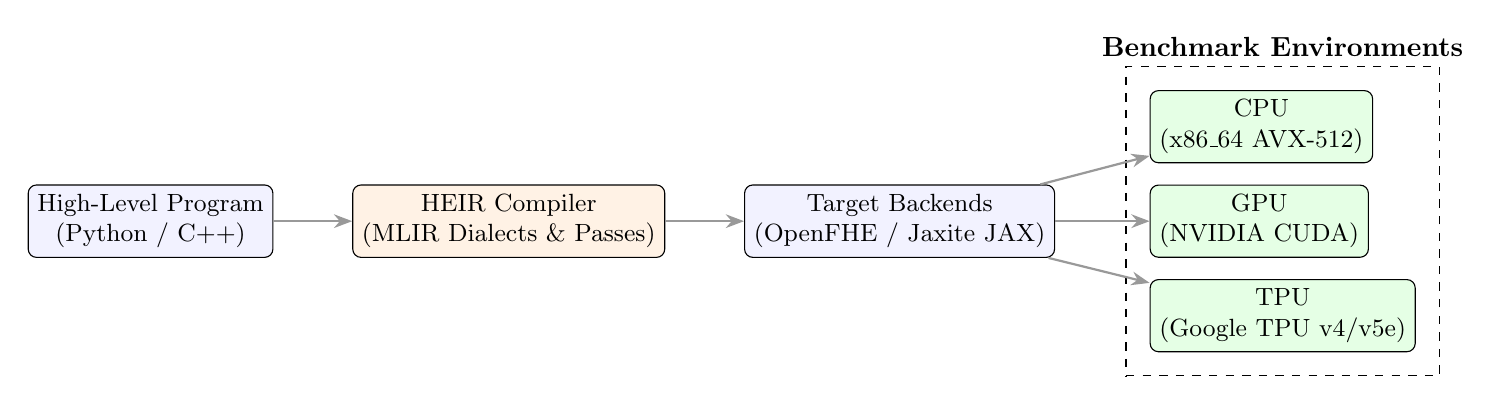
\begin{tikzpicture}[
    node distance=1.3cm and 1.0cm,
    box/.style={draw, rectangle, rounded corners=3pt, align=center, minimum height=0.9cm, minimum width=2.4cm, fill=blue!5, font=\small},
    mlirbox/.style={draw, rectangle, rounded corners=3pt, align=center, minimum height=0.9cm, minimum width=2.4cm, fill=orange!10, font=\small},
    hwbox/.style={draw, rectangle, rounded corners=3pt, align=center, minimum height=0.8cm, minimum width=2.0cm, fill=green!10, font=\small},
    arrow/.style={-Stealth, thick, draw=gray!80}
]

% Nodes
\node (src) [box] {High-Level Program\\(Python / C++)};
\node (heir) [mlirbox, right=of src] {HEIR Compiler\\(MLIR Dialects \& Passes)};
\node (codegen) [box, right=of heir] {Target Backends\\(OpenFHE / Jaxite JAX)};

% Hardware Targets
\node (cpu) [hwbox, right=1.2cm of codegen, yshift=1.2cm] {CPU\\(x86\_64 AVX-512)};
\node (gpu) [hwbox, right=1.2cm of codegen, yshift=0cm] {GPU\\(NVIDIA CUDA)};
\node (tpu) [hwbox, right=1.2cm of codegen, yshift=-1.2cm] {TPU\\(Google TPU v4/v5e)};

% Benchmarking Container
\node (bench) [draw, dashed, inner sep=0.3cm, fit=(cpu) (gpu) (tpu), label=above:\textbf{Benchmark Environments}] {};

% Connections
\draw [arrow] (src) -- (heir);
\draw [arrow] (heir) -- (codegen);
\draw [arrow] (codegen) -- (cpu);
\draw [arrow] (codegen) -- (gpu);
\draw [arrow] (codegen) -- (tpu);

\end{tikzpicture}
\caption{System Architecture Overview: Decoupling high-level algorithm logic from FHE hardware targets using the HEIR compiler framework.}
\label{fig:system_architecture}
\end{figure}

\newpage

In plain-texts, sorting and shuffling rely on conditional branching (e.g., \texttt{if (A > B)}) and array indexing based on secret data. In Fully Homomorphic Encryption, conditional branching on cipher-texts is strictly prohibited because data values cannot be leaked to the execution environment. Consequently, operations must be reformulated as data-oblivious arithmetic circuits. 

\subsubsection{Encrypted List Sorting}
To evaluate HEIR's ability to compile comparison-heavy logic, we implement a \textbf{Bitonic Sorting Networks} \cite{1993icpp....1...23L}. Standard comparison algorithms ($O(N \log N)$ average complexity) exhibit input-dependent branch execution paths. Bitonic Sorting transforms the sorting process into a fixed sequence of Compare-and-Swap (CAS) units:

\begin{equation}
\text{CAS}(x, y) = \Big( \text{min}(x,y),, \text{max}(x,y) \Big)
\end{equation}

In an encrypted domain, $\text{min}(x,y)$ and $\text{max}(x,y)$ are computed using homomorphic sign evaluators or polynomial approximations:
\begin{align}
\text{min}(x, y) &= \frac{x + y - |x - y|}{2} \
\text{max}(x, y) &= \frac{x + y + |x - y|}{2}
\end{align}

Bitonic sorting networks enforce a fixed computational depth of $O(\log^2 N)$ and a total of $O(N \log^2 N)$ comparisons regardless of data permutation. Cheon et al., 2019; Gouert et al., 2023) demonstrate that Bitonic sorting is a standard benchmark for testing multiplicative depth and  overheads in Homomorphic encryption compilers.

\subsubsection{Encrypted List Shuffling}
Permuting data homomorphically without revealing the permutation pattern requires \textbf{Oblivious Permutation Networks} (such as Waksman or Bene\v{s} routing networks). While both Bene\v{s} and Waksman networks realize $O(N \log N)$ permutations in identical stage depth ($2\lceil \log_2 N \rceil - 1$), we  select the Bene\v{s} network over the Waksman network for our HEIR compiler implementation based on the following cryptographic and compiler optimization principles:

\begin{itemize}
\item \textbf{Structural Symmetry and SIMD Lowering:} A Bene\v{s} network is constructed by concatenating two mirrored, identical sub-networks. Every stage features uniform layout and constant lengths. In contrast, a Waksman network eliminates redundant $2 \times 2$ switches ($\approx N/2$ switches saved total). Because MLIR dialect transformations rely on structured patterns to enable SIMD slot vectorization, the strict topological regularity of Bene\v{s} networks lowers significantly better through MLIR loop passes.
\item \textbf{Multiplicative depth:} In FHE, the primary computational bottleneck is multiplicative depth. Waksman's switch reduction reduces the total count of addition/multiplication operations by $\approx N/2$, but it does not decrease the overall depth of the network. Since both networks require the exact same multiplicative depth, Waksman provides no advantage.
\item \textbf{Hardware Accelerator Portability (GPU/TPU):} When lowering code via HEIR to Jaxite or OpenFHE, execution performance on GPUs and TPUs is bottlenecked by memory throughput. The highly symmetric vector permutation in a Bene\v{s} network enable optimal parallel dispatch on NVIDIA CUDA and Google TPU execution pipelines.
\end{itemize}

A Bene\v{s} network consists of $(2\lceil \log_2 N \rceil - 1)$ stages of $2 \times 2$ routing switches. Each switch performs a homomorphic multiplexing operation conditioned on a control bit $s \in \{0, 1\}$:\begin{align}out_0 &= (1 - s) \cdot in_0 + s \cdot in_1 \\out_1 &= s \cdot in_0 + (1 - s) \cdot in_1\end{align}When control bits $s$ are known to the evaluator or pre-computed (plaintext control bits), the switches perform low-noise Ciphertext $\times$ Plaintext operations, maintaining a overall multiplicative depth bounded by $2\lceil \log_2 N \rceil - 1$.

\subsection{Work so far}                                 % 2 pages max
\secinfo{Joris}{Jimena}

Our implementation relies on the compiler infrastructure established in \cite{ali2025heir}. By providing an abstraction layer that decouples application logic from a specific cryptographic back-end, their work supplies the tool chain we use to compile our sorting and shuffling algorithms.

To anticipate the hardware bottlenecks we are going to face in this project, we look at the benchmarking already done in \cite{bian2023heir}. Although this is a different HEIR framework, by coincidence with the same name, this paper exposes a fundamental limitation inherent to FHE. Bit wise operations will cause memory usage to scale exponentially. Our work will rely mostly on bitwise operation, so from this we are estimating that we will hit a memory wall long before we hit a computational wall.

The problem is that if you use MPC too much the memory wall will come down, but the communication wall will rise. Every non-linear MPC calculation brings communication and this will throttle the workings, as shuffling and sorting are non-linear algorithms. In the paper Beyond Latency: A System-Level Characterization of MPC and FHE for PPML \cite{huang2026beyond} the specific point where FHE and MPC meet in efficiency is found. This paper, however,  primarily focuses on PPML, which is dominated by linear matrix multiplications. Hence their findings will not directly map to ours as we will have mostly bit wise operations. This paper does give us a very rigorous framework to work from if we adapt it to our needs.

Finally we look at the paper "A Pragmatic Comparison of Cryptographic Computation Technologies for Machine Learning" \cite{taubert2026pragmatic}. This establishes the pragmatic flaws in a real life system such as latency and how it effects the viability of the system. Which means the viability will be heavily dependent on close proximity networks and will be severely penalized over long distance networking.


\subsection{Ambition}                                    % 1/2 page max
\secinfo{Joris}{Louis Nathan}
Looking at the papers we seem to be the first ones that are evaluating the HEIR framework through a pure shuffling and sorting stance and not a machine learning stance. Having an empirical number quantifying its efficiency would help future research. 

\subsection{Related work}                                % 2 pages max
\secinfo{Joris}{Louis Nathan}

So why will our research be better than an existing solution? The related work so far is quite scarce, HEIR being a relatively newly introduced framework. Because if this there is still need for comprehensive, independent benchmarking of its cross platform performance.

As referred to in the work so far chapter most of the studies done have focussed privacy preserving machine learning. In the papers "beyond latency" \cite{huang2026beyond} and "a pragmatic comparison of cryptographic computation technologies" \cite{taubert2026pragmatic} system level characterizations and latency evaluations are provided. However theses are focused on linear operations. Moving the focus to non linear operations will expose different limitations of the framework.

So the reasons why our approach will be better for this specific goal is that we have targeted stress testing. Instead of blending linear and non linear task we will purely focus on the bit wise memory bottlenecks identified in existing literature. This should push the HEIR compiler to its absolute theoretical limit. Because we don't use highly optimized linear operations we will have a more unadulterated metric on how efficient the compiler handles complex control flow constraints.


